\documentclass[11pt,a4paper]{article}
\usepackage[utf8]{inputenc}
\usepackage[T1]{fontenc}
\usepackage[english]{babel}
\usepackage[margin=2.1cm]{geometry}
\usepackage{booktabs,array,tabularx}
\usepackage{xcolor}
\usepackage{graphicx}
\usepackage{pgfplots}
\pgfplotsset{compat=1.17}
\PassOptionsToPackage{hyphens}{url}
\usepackage[hidelinks]{hyperref}
\usepackage{enumitem}
\setlist{nosep,leftmargin=1.4em}
\emergencystretch=3em

\definecolor{impl}{HTML}{3B6EA8}
\definecolor{rev}{HTML}{8FB3DA}

\title{Sweatshop on P-Chess: the v0.1.0 game-screen tickets\\\large Resign button and Reason header (UI-013), draw offers (BOT-011), match score (UI-014), board resize grip (UI-015) and the repertoire snapshot file (HIST-003); GPT-6.1 Terra lineup, lane \texttt{v010}}
\author{Foreman, session \texttt{sweatshop/v010/2026-10-30-1831}}
\date{30 October 2026}

\begin{document}
\maketitle

\section*{Summary}

A lane run (\texttt{-Lane v010}) in a fresh clone at \path{.artifacts-build/lanes/v010}, default
lineup \texttt{terra}: stage 2 on \texttt{gpt-6.1-terra high}, hard tickets on
\texttt{gpt-6.1-terra xhigh} (BOT-011), review on \texttt{gpt-6.1-sol xhigh}. The lanes
\texttt{analysis} and \texttt{repertoire} ran at the same time in their own clones. Before launch
the clone's gate passed (270 passed, 0 failed) with the Lc0 binary and Maia nets copied in.
Launch at 18:31, last merge at 20:02.

\begin{itemize}
  \item \textbf{Produced:} UI-013, BOT-011, UI-014, UI-015 and HIST-003 merged on the session,
        \texttt{Verdict: Approve}, all \texttt{Review: agent}. Session PR
        \href{https://github.com/Laginho/P-Chess/pull/27}{\#27}. Gate 287 passed, 0 failed
        (270 before the run).
  \item \textbf{Cost:} \textbf{\$7.05} at API list price over the 8 priced stages (all reviews,
        \texttt{gpt-6.1-sol xhigh}); the 7 Terra stages log \texttt{?} (no Terra row in the
        driver's \texttt{\$CodexPrices}). Codex quota: 6 points of the weekly window (Terra high
        3, Terra xhigh 1, Sol 2, each $\pm$1), in a window shared with the two concurrent lanes.
  \item \textbf{What went wrong:} UI-013 and UI-014 were reopened once each, two real P2
        findings each. HIST-003's first review stopped on a scope question the driver does not
        relay to the proxy; the foreman asked it and relaunched.
  \item \textbf{Paused, by design:} the other nine \texttt{v010} tickets wait on the
        \texttt{analysis} lane: REV-005 on REV-002 and REV-003, REV-006, HIST-004 and UI-019 on
        REV-004, HIST-006 on REV-002, the rest behind HIST-004. They become runnable when
        \href{https://github.com/Laginho/P-Chess/pull/26}{PR \#26} is merged and a new
        \texttt{v010} session starts.
  \item \textbf{Provisional verdict:} Terra is fast (median 8~min per first stage 2, 4--6~min
        per fix) and keeps test-first commits, but its first attempt on UI tickets misses state
        interactions around the feature. Under 10 reviews, an anecdote.
\end{itemize}

\section*{What was done}

\textbf{UI-013}: a flag button between the clocks resigns the game; the first click arms it
(``Click again to resign''), a second click within 2~s resigns, and it shares one arming window
with \texttt{Esc}. Every saved PGN gains a \texttt{Reason} header (checkmate, resignation, time,
\dots). Main files \path{ui/main.gd}, \path{ui/main.tscn}, \path{core/pgn.gd}. Reopened once:
the button showed \texttt{?} instead of a flag, because Terra wrote the glyph through a
\texttt{python -c} edit inside PowerShell and the codepage replaced it (\path{ui/main.tscn});
and a clicked button kept keyboard focus, so with Settings open \texttt{Space} resigned the
game behind the modal (\path{ui/main.gd}).

\textbf{BOT-011}: a \textonehalf{} button offers Maia a draw. Maia answers with its next move
from its own search evaluation (Lc0's \texttt{score cp}, verified first and recorded in the
ticket) and a deterministic rule on material and its clock; ``Draw agreed'' ends the game as a
draw by agreement (PGN \texttt{Reason: agreement}, stats count a draw), ``Maia declined'' plays
its move. The button rests for ten of your moves after an offer. The rule's numbers live in the
new \path{core/tunables.gd}. Main files \path{engine/uci.gd}, \path{bot/maia_player.gd},
\path{ui/main.gd}. Merged at the first review.

\textbf{UI-014}: rematches keep a match score: a win counts 1, a draw \textonehalf{} each; the
game-over panel shows ``You 2 -- 1 Maia 1500'', and from the first rematch each clock row
carries that player's score in a small box that follows the colour swap. New game, a changed
setting or an engine stop reset it. Main file \path{ui/main.gd}. Reopened once: after a finished
rematch the boxes still showed the previous score (set only at game start), and they stayed
visible in F11 focus mode, which shows only board and clocks (\path{ui/main.gd}).

\textbf{UI-015}: a grip on the board's bottom-right corner drags the board bigger or smaller; it
stays square, is clamped to a minimum and to the window, the size is saved in the
\texttt{board\_size} setting, and a double-click returns to fit-to-window. Main files
\path{ui/resize_grip.gd} (new), \path{core/settings.gd}. Merged at the first review.

\textbf{HIST-003}: a game played with a repertoire loaded now saves the lines it was checked
against beside its PGN, as \texttt{<game>.repertoire.json}, with the repertoire's colour, so a
review opened later from the history (HIST-004) checks against that snapshot and not against
today's repertoire. A failed snapshot write reports like a failed PGN write. Main file
\path{core/history.gd}. No defect found; the first review stopped only to ask whether the
reader function and the colour capture were inside the ticket's Primary files (they were in
named files, required by criteria 4 and 1); the proxy approved and the re-review merged it.

\section*{Timeline}

\begin{tabularx}{\linewidth}{@{}lX@{}}
\toprule
18:31 & Clone of \texttt{origin} at \texttt{eea8c16}; gate 270/0; launch, pid 6924. \\
18:41 & UI-013 to review (Terra high, 9~min). \\
18:46 & UI-013 reopened, 2 findings. Stage 2 again. \\
18:50 & UI-013 to review (4~min). \\
18:54 & UI-013 merged. BOT-011 stage 2 (Terra xhigh, hard). \\
19:03 & BOT-011 to review (9~min). \\
19:09 & BOT-011 merged, 0 findings. UI-014 stage 2. \\
19:17 & UI-014 to review (8~min). \\
19:22 & UI-014 reopened, 2 findings. Stage 2 again. \\
19:28 & UI-014 to review (6~min). \\
19:32 & UI-014 merged. UI-015 stage 2. \\
19:40 & UI-015 to review (8~min). \\
19:44 & UI-015 merged, 0 findings. HIST-003 stage 2. \\
19:50 & HIST-003 to review (6~min). \\
19:54 & HIST-003 review ends at \texttt{blocked} (scope question, proxy unreachable from Codex). Driver: nothing runnable; PR \#27 opened (4 tickets). \\
19:55 & Foreman asks the proxy: Approve. Recorded on the session (\texttt{573eaa1}) and the ticket branch; \texttt{to-review} restored. \\
19:56 & Relaunch, pid 30484. \\
20:02 & HIST-003 merged, 0 findings; nothing runnable; PR \#27 updated (5 tickets). \\
\bottomrule
\end{tabularx}

\section*{Per stage}

{\small
\begin{tabularx}{\linewidth}{@{}llllrrrrrX@{}}
\toprule
When & Ticket & Stage & Model & Min & In & Cache & Out & Cost & Outcome \\
\midrule
18:41 & UI-013 & impl & terra high & 9 & 3.1M & 97\% & 10k & ? & to-review \\
18:46 & UI-013 & review & sol xhigh & 5 & 3.4M & 95\% & 14k & 1.13 & reopened \\
18:50 & UI-013 & impl & terra high & 4 & 1.7M & 94\% & 5k & ? & to-review \\
18:54 & UI-013 & review & sol xhigh & 4 & 1.8M & 93\% & 10k & 0.68 & merged \\
19:03 & BOT-011 & impl & terra xhigh & 9 & 7.6M & 98\% & 19k & ? & to-review \\
19:09 & BOT-011 & review & sol xhigh & 6 & 3.7M & 95\% & 15k & 1.21 & merged \\
19:17 & UI-014 & impl & terra high & 8 & 3.7M & 98\% & 10k & ? & to-review \\
19:22 & UI-014 & review & sol xhigh & 5 & 2.7M & 94\% & 14k & 0.96 & reopened \\
19:28 & UI-014 & impl & terra high & 6 & 2.7M & 97\% & 6k & ? & to-review \\
19:32 & UI-014 & review & sol xhigh & 4 & 1.9M & 91\% & 12k & 0.79 & merged \\
19:40 & UI-015 & impl & terra high & 8 & 3.6M & 98\% & 11k & ? & to-review \\
19:44 & UI-015 & review & sol xhigh & 4 & 2.2M & 94\% & 13k & 0.81 & merged \\
19:50 & HIST-003 & impl & terra high & 6 & 2.9M & 96\% & 8k & ? & to-review \\
19:54 & HIST-003 & review & sol xhigh & 3 & 2.0M & 92\% & 12k & 0.80 & blocked \\
20:02 & HIST-003 & review & sol xhigh & 5 & 2.5M & 94\% & 13k & 0.66 & merged \\
\midrule
 & & & & 86 & 45.5M & & 172k & 7.05+? & \\
\bottomrule
\end{tabularx}
}

\begin{center}
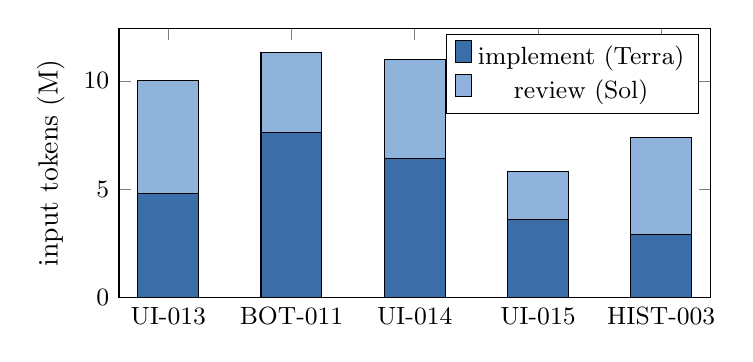
\begin{tikzpicture}
\begin{axis}[ybar stacked, bar width=22pt, width=0.75\linewidth, height=5cm,
  symbolic x coords={UI-013,BOT-011,UI-014,UI-015,HIST-003},
  xtick=data, ylabel={input tokens (M)}, ymin=0, legend style={at={(0.98,0.98)},anchor=north east,font=\small},
  tick label style={font=\small}]
\addplot[fill=impl] coordinates {(UI-013,4.8) (BOT-011,7.6) (UI-014,6.4) (UI-015,3.6) (HIST-003,2.9)};
\addplot[fill=rev] coordinates {(UI-013,5.2) (BOT-011,3.7) (UI-014,4.6) (UI-015,2.2) (HIST-003,4.5)};
\legend{implement (Terra), review (Sol)}
\end{axis}
\end{tikzpicture}
\end{center}

The chart is input tokens, not dollars: Terra's stages are unpriced. Wasted: the two reopen
rounds (UI-013 3.1M + 3.4M, UI-014 3.7M + 2.7M in the rejected first attempt and its review)
and HIST-003's blocked first review (2.0M in, \$0.80), whose question needed no code change.

\section*{Comparison with previous runs}

From \texttt{run-log.md}: Terra's first stage 2 on the four normal tickets took 6--9~min
(median 8), the fixes after a reopen 4--6~min. Over its P-Chess history
\texttt{gpt-6.1-sol high} took a median of 11~min per first stage 2 (21 runs, 0 failed). The
hard ticket on \texttt{gpt-6.1-terra xhigh} took 9~min, against 11--17~min for the three hard
tickets on \texttt{gpt-6.1-sol xhigh} in the 27 October QA lane. Token volumes are comparable
(Terra 1.7--7.6M in, 5--19k out; Sol high 2--5M in, 10--28k out). Reviews cost about the same as
on 27 October (\$0.66--1.21 now, \$0.75--0.79 then); the dearest are the reopening reviews and
BOT-011's. The same-day \texttt{repertoire} lane (also Terra) reopened 1 of 3 tickets, with
four findings.

\section*{Observations per model}

\begin{itemize}
  \item \textbf{gpt-6.1-terra high, stage 2} (6 stages): every ticket opens with a
        \texttt{test:} commit before its production commit, and both reopen fixes started
        with a red regression test that followed the reviewer's request (UI-013's dispatches
        real viewport input). Diffs stay small (+59 to +129 lines) and fixes are tightly
        scoped (+33 and +46 lines), with no scope creep. It never asked the proxy, never failed
        the gate, and disclosed manual acceptance honestly in every handoff. Weak spots:
        (1)~\emph{state around the feature}: UI-013 missed the Settings modal, UI-014 the
        result update and F11, all paths the repo already guards for other controls;
        (2)~\emph{non-ASCII through the shell}: UI-013's flag became \texttt{?}; it caught the
        same trap itself on BOT-011 (a label test, then a fix) and UI-014 (code points), but
        UI-014's fix commit and its later score-box commit carry no test of their own;
        (3)~UI-015's grip-interaction test came after its feature commit (proved by a disclosed
        mutation check, not a red run); (4)~HIST-003 widened the Primary-file scopes silently;
        a one-line note in the handoff would have spared the blocked review. Branch names
        vary per ticket (\texttt{ui-013}, \texttt{BOT-011-draw-offer},
        \texttt{UI-014-match-score}, \texttt{HIST-003}); the helper accepts all of them.
  \item \textbf{gpt-6.1-terra xhigh, stage 2} (BOT-011, 1 stage): the strongest stage of the
        run: six red/green pairs, the ticket's ``verify first'' step on Lc0's \texttt{score cp}
        done and recorded before the rule, merged with 0 findings in 9~min.
  \item \textbf{gpt-6.1-sol xhigh, review} (8 stages, 3--6~min): each review checked the
        red/green order and reused the gate receipt after checking hash and code; both
        reopening reviews reproduced their findings with headless probes through real input,
        and both re-reviews raised nothing new (no drip-feed). The only code written in review
        was a comment (BOT-011's reason list), so no round-0 rows. HIST-003's first review
        stopped correctly on a contract question but could not reach the proxy.
\end{itemize}

\section*{Driver and runtime issues}

\begin{enumerate}
  \item \texttt{\$CodexPrices} has no \texttt{gpt-6.1-terra} row: every Terra stage logs
        \texttt{?}, so the lineup's cost still cannot be compared (also reported by the
        \texttt{repertoire} lane).
  \item A stage-3 question is not relayed to the proxy: the driver puts stage-2 questions to
        the proxy, but a review that ends \texttt{blocked} with the proxy unreachable (Codex
        sandbox) is left ``for a human''. Here the foreman asked and relaunched (one extra
        driver start, about 2~min).
  \item Codex stages' \texttt{.txt.err} files fill with ``Reading additional input from
        stdin\dots''; noise, no effect on the run.
  \item Shutdown 1.0--2.6~s per stage; no crash, no timeout, no retry.
\end{enumerate}

\section*{Recommendations}

\begin{enumerate}
  \item Add a \texttt{gpt-6.1-terra} row to \texttt{\$CodexPrices} before the next Terra run.
  \item Have the driver relay a blocked stage-3 question to the proxy as it does for stage 2
        (twice per ticket per run), so a scope question does not end the run.
  \item For UI tickets, add to the ticket's test list the state paths around the new control:
        Settings open, F11 focus mode, rematch and game end. Both reopens of this run, and
        OPEN-007's in the \texttt{repertoire} lane, were of that kind.
  \item Keep Terra as default for \texttt{normal} tickets until ten reviews: scoreboard row
        \texttt{gpt-6.1-terra high} $\rightarrow$ \texttt{gpt-6.1-sol xhigh}, 9 reviews,
        3 reopened (33\%), S2 rate 33\% --- an anecdote, against \texttt{gpt-6.1-sol high}
        $\rightarrow$ \texttt{gpt-6.1-sol xhigh}, 18 reviews, 22\%. Terra is faster per stage;
        whether it is cheaper waits on recommendation~1.
  \item Before a release, play the manual checks below; every ticket of this run left product
        acceptance pending.
\end{enumerate}

\section*{Human debt and proxy decisions}

No \texttt{Débito humano:} lines in this run's tickets. One proxy decision, on HIST-003,
asked by the foreman after the review blocked:

\begin{itemize}
  \item \texttt{Proxy decided (opus-5.5 xhigh)}: ``Approve. Criterion 4 requires the reader and
        criterion 1 requires the colour, so both edits are authorized. Stage 1 does not need to
        clarify anything first. Fold the widened scopes below into Primary files so the
        boundary matches what was merged - both edits sit in files the ticket already names,
        and the numbered criteria require them.''
\end{itemize}

\section*{Reopen attribution}

Labelled by the foreman (opus-5.5); the reviewer was \texttt{gpt-6.1-sol xhigh}, so no
self-judging. Rows appended to \path{.scratch/reopen-attribution.md}.

{\small\noindent
\begin{tabularx}{\linewidth}{@{}>{\raggedright\arraybackslash}p{1.6cm}X>{\raggedright\arraybackslash}p{2.7cm}X@{}}
\toprule
Ticket (round) & Finding & Label & Why \\
\midrule
UI-013 (1) & Resign button shows \texttt{?} instead of a flag & S2-explícito/\allowbreak código & criterion 1; the glyph was lost in the shell and the scene never read back \\
UI-013 (1) & Focused button + Settings open + \texttt{Space} resigns behind the modal & S2-implícito & regression of stage 2's own focusable button against the existing Settings barrier \\
UI-014 (1) & Clock-row boxes keep the previous score after a finished rematch & S2-explícito/\allowbreak código & criterion 3 and the ticket's test list; the test checked the panel only \\
UI-014 (1) & Score boxes visible in F11 focus mode & S2-implícito & regression against spec focus mode, a convention other controls follow \\
\bottomrule
\end{tabularx}
}

Totals: S2-explícito/código 2, S2-implícito 2, S1 0, S3-ruído 0. No review miss, no
review-induced churn, no fix made in review. HIST-003's blocked review is not a reopen and has no
row. No session-review, release-audit or post-release finding: the Copilot reviewer on PR \#27
did not run (out of quota), which says nothing about defects.

\section*{Scoreboard}

\texttt{scoreboard.ps1} over the ClassyCall, EasyMath, PhysiSyst, SIGAA-ME and SynchroNice main
checkouts, plus this lane's clone in place of P-Chess's main checkout (same merged run log, and
it holds this run's attribution rows before they reach \texttt{main}). Moved since the
\texttt{repertoire} report of the same day: implementer \texttt{gpt-6.1-terra high} 4 $\to$ 10
stage runs (9 to review, 1 failed, median 8~min); new row \texttt{gpt-6.1-terra xhigh}, 1 run;
pair \texttt{gpt-6.1-terra high} $\rightarrow$ \texttt{gpt-6.1-sol xhigh} 3 $\to$ 9 reviews,
1 $\to$ 3 reopened, rate unchanged at 33\% (anecdote); findings row 3 rounds, 5 S2-explicit
code, 3 S2-implicit; new interventions row \texttt{proxy-decision (opus-5.5 xhigh)} 1.

{\tiny
\begin{verbatim}
| Implementer | Stage runs | To review | Failed | Asked | Median min to review | Cost |
|---|---|---|---|---|---|---|
| gpt-6.1-sol high | 64 | 59 | 0 | 5 | 9m | $49.27 (64/64 priced) |
| opus-5.5 medium | 3 | 2 | 1 | 0 | 6m | $4.79 (3/3 priced) |
| opus-5.5 | 7 | 4 | 0 | 3 | 14m | $15.12 (7/7 priced) |
| gpt-6-luna max | 89 | 61 | 10 | 18 | 17m | $4.91 (85/89 priced) |
| sonnet-5.5 high | 2 | 2 | 0 | 0 | 7m | $3.77 (2/2 priced) |
| gpt-6-astra high | 1 | 0 | 0 | 1 | - | $3.92 (1/1 priced) |
| opus-5.5 xhigh | 18 | 14 | 4 | 0 | 12m | $91.78 (18/18 priced) |
| gpt-6.1-sol max | 6 | 5 | 0 | 1 | 24m | $12.12 (6/6 priced) |
| haiku-5.5 high | 2 | 0 | 2 | 0 | - | $1.00 (2/2 priced) |
| opus-5.5 high | 20 | 13 | 6 | 1 | 6m | $37.46 (20/20 priced) |
| gpt-6.1-sol xhigh | 9 | 9 | 0 | 0 | 12m | $9.84 (9/9 priced) |
| gpt-6.1-terra high | 10 | 9 | 1 | 0 | 8m | ? |
| gpt-6.1-terra xhigh | 1 | 1 | 0 | 0 | 9m | ? |
| gpt-6-sol xhigh | 1 | 1 | 0 | 0 | 9m | $0.40 (1/1 priced) |
| fable | 1 | 1 | 0 | 0 | 11m | ? |
| gpt-6-luna | 8 | 4 | 4 | 0 | 37m | ? |
| gpt-6-sol | 6 | 5 | 1 | 0 | 17m | ? |
| gpt-5.6-sol | 5 | 4 | 1 | 0 | 17m | ? |
| gpt-6-astra | 18 | 11 | 6 | 1 | 8m | ? |
| sonnet | 5 | 3 | 2 | 0 | 14m | $10.53 (4/5 priced) |
| sonnet-5 xhigh | 11 | 6 | 2 | 3 | 8m | $18.09 (11/11 priced) |

| Implementer | Reviewer | Reviews | Reopened | Reopen rate | Reopened for S2 | S2 rate | Unclassified | Fixed in review for S2 |
|---|---|---|---|---|---|---|---|---|
| gpt-6.1-sol high | gpt-6.1-sol max | 38 | 12 | 32% | 9 | >=24% | 2 | 1 |
| opus-5.5 medium | gpt-6.1-sol max | 2 | 1 | 50% | 0 | >=0% | 1 | 0 |
| opus-5.5 | opus-5.5 | 4 | 0 | 0% | 0 | 0% | 0 | 0 |
| gpt-6-luna max | opus-5.5 high | 18 | 1 | 6% | 1 | 6% | 0 | 0 |
| gpt-6-luna max | gpt-6-sol max | 43 | 23 | 53% | 22 | 51% | 0 | 0 |
| ? | gpt-6-sol max | 1 | 0 | 0% | 0 | 0% | 0 | 0 |
| sonnet-5.5 high | gpt-6-sol max | 2 | 1 | 50% | 1 | 50% | 0 | 0 |
| opus-5.5 xhigh | gpt-6.1-sol max | 6 | 3 | 50% | 3 | 50% | 0 | 0 |
| ? | gpt-6.1-sol max | 1 | 0 | 0% | 0 | 0% | 0 | 0 |
| gpt-6.1-sol max | gpt-6.1-sol max | 4 | 1 | 25% | 1 | 25% | 0 | 0 |
| ? | opus-5.5 xhigh | 4 | 1 | 25% | 1 | 25% | 0 | 0 |
| opus-5.5 xhigh | opus-5.5 xhigh | 7 | 0 | 0% | 0 | 0% | 0 | 0 |
| opus-5.5 high | opus-5.5 xhigh | 10 | 2 | 20% | 2 | 20% | 0 | 3 |
| gpt-6.1-sol high | gpt-6.1-sol xhigh | 18 | 4 | 22% | 4 | 22% | 0 | 0 |
| gpt-6.1-sol xhigh | gpt-6.1-sol xhigh | 9 | 1 | 11% | 1 | 11% | 0 | 1 |
| gpt-6.1-terra high | gpt-6.1-sol xhigh | 9 | 3 | 33% | 3 | 33% | 0 | 0 |
| ? | gpt-6.1-sol xhigh | 1 | 0 | 0% | 0 | 0% | 0 | 0 |
| gpt-6.1-terra xhigh | gpt-6.1-sol xhigh | 1 | 0 | 0% | 0 | 0% | 0 | 0 |
| gpt-6-sol xhigh | gpt-6-astra high | 1 | 0 | 0% | 0 | 0% | 0 | 0 |
| fable | fable | 1 | 1 | 100% | 0 | >=0% | 1 | 0 |
| ? | opus | 1 | 0 | 0% | 0 | 0% | 0 | 0 |
| gpt-6-luna | gpt-6-sol | 4 | 4 | 100% | 0 | >=0% | 4 | 0 |
| gpt-6-sol | gpt-5.6-sol | 5 | 4 | 80% | 0 | >=0% | 4 | 0 |
| gpt-5.6-sol | gpt-6-astra | 4 | 3 | 75% | 0 | >=0% | 3 | 0 |
| gpt-6-astra | gpt-5.6-sol | 11 | 5 | 45% | 0 | >=0% | 5 | 0 |
| sonnet | opus | 3 | 1 | 33% | 1 | 33% | 0 | 0 |
| sonnet-5 xhigh | opus-5.5 xhigh | 5 | 0 | 0% | 0 | 0% | 0 | 0 |

| Implementer -> Reviewer | Rounds | S2 explicit code | S2 explicit test | S2 implicit | S1 | S3 noise |
|---|---|---|---|---|---|---|
| gpt-6-astra medium -> gpt-6.1-sol max | 8 | 11 | 1 | 4 | 1 | 0 |
| gpt-6.1-sol-fast high -> gpt-6.1-sol-fast max | 2 | 2 | 0 | 0 | 0 | 0 |
| gpt-6.1-sol-fast max -> gpt-6.1-sol-fast max | 6 | 2 | 0 | 3 | 1 | 0 |
| gpt-6.1-sol high -> gpt-6.1-sol max | 26 | 16 | 4 | 23 | 1 | 0 |
| gpt-6-luna max -> opus-5.5 high | 1 | 1 | 1 | 0 | 1 | 0 |
| gpt-6-luna max -> gpt-6-sol max | 23 | 31 | 3 | 23 | 12 | 15 |
| sonnet-5.5 high -> gpt-6-sol max | 1 | 3 | 0 | 2 | 0 | 0 |
| opus-5.5 xhigh -> gpt-6.1-sol max | 3 | 3 | 0 | 2 | 1 | 0 |
| gpt-6.1-sol max -> gpt-6.1-sol max | 5 | 7 | 0 | 5 | 0 | 0 |
| haiku-5.5 high -> gpt-6.1-sol max | 3 | 3 | 1 | 5 | 1 | 0 |
| gpt-6.1-sol high -> gpt-6.1-sol xhigh | 53 | 53 | 4 | 23 | 3 | 0 |
| gpt-6.1-sol max -> gpt-6.1-sol xhigh | 2 | 0 | 0 | 3 | 0 | 0 |
| opus-5.5 high -> opus-5.5 xhigh | 8 | 7 | 0 | 3 | 0 | 0 |
| gpt-6.1-sol xhigh -> gpt-6.1-sol xhigh | 3 | 4 | 0 | 1 | 0 | 0 |
| opus-5.5 high -> gpt-6.1-sol xhigh | 1 | 2 | 0 | 0 | 0 | 0 |
| gpt-6.1-terra high -> gpt-6.1-sol xhigh | 3 | 5 | 0 | 3 | 0 | 0 |
| sonnet-5.5 high -> gpt-6.1-sol max | 3 | 5 | 0 | 2 | 3 | 0 |
| sonnet-5.5 xhigh -> gpt-6.1-sol max | 3 | 7 | 0 | 3 | 2 | 0 |
| sonnet-5.5 high -> opus-5.5 xhigh | 3 | 1 | 2 | 0 | 0 | 0 |
| gpt-6-astra medium -> gpt-6-astra xhigh | 1 | 1 | 0 | 0 | 0 | 0 |
| fable -> ? | 4 | 5 | 1 | 3 | 1 | 0 |
| sonnet -> ? | 10 | 3 | 6 | 9 | 3 | 2 |
| opus -> ? | 1 | 3 | 0 | 0 | 0 | 0 |
| sonnet? -> ? | 11 | 3 | 4 | 12 | 3 | 5 |
| sonnet -> opus | 1 | 1 | 1 | 0 | 0 | 0 |
| gpt-6-astra low -> gpt-6.1-sol max | 1 | 2 | 0 | 1 | 0 | 0 |

Evidence coverage: legacy flags and absent records are unknown, not zero defects or zero interventions.
| Discovery | Recorded findings | Earlier review miss (yes / known) | Review-induced churn (yes / known) |
|---|---|---|---|
| ticket-review | 372 | 5 / 177 | 1 / 179 |
| session-review | 28 | 22 / 24 | 0 / 27 |
| release-audit | 2 | 2 / 2 | 0 / 2 |
Runtime completion to process exit: 240.316s total over 196 measured stages; 333 unmeasured.
| Intervention | Recorded events |
|---|---|
| human-rescue | 30 |
| automatic-recovery | 89 |
| proxy-decision (unknown) | 37 |
| routine-approval | 18 |
| proxy-decision (gpt-6-astra high, fallback) | 58 |
| proxy-decision (opus) | 42 |
| proxy-decision (supervisor) | 12 |
| proxy-decision (opus-5.5 xhigh) | 1 |
\end{verbatim}
}

\section*{Pending for the human}

\begin{enumerate}
  \item UI-013: resign with two clicks; let the hint expire and check one click only arms;
        click then \texttt{Esc} and \texttt{Esc} then click; open Settings after arming and press
        \texttt{Space} (nothing happens); check the flag renders.
  \item BOT-011: offer a draw in the opening (declined) and in a dead-equal endgame with low
        clocks (accepted); check the \textonehalf{} button, the notice and the side panel.
  \item UI-014: win, rematch, draw, rematch: the panel reads 1\textonehalf{} -- \textonehalf{}
        and the boxes follow the colours; F11 hides them.
  \item UI-015: drag the grip, restart, check the saved size; double-click returns to
        fit-to-window; check the cursor and the layout.
  \item HIST-003: nothing to play now; its product check is HIST-004's criterion 6.
  \item Review and merge session PR \#27. Then merge \texttt{analysis}'s PR \#26 and relaunch
        the \texttt{v010} lane for the nine waiting tickets, and tell the other open lanes'
        foremen to sync.
\end{enumerate}

\end{document}
